%
% $RCSfile: whole_part.tex,v $
%
% Copyright (C) 2002-2008. Christian Heller.
%
% Permission is granted to copy, distribute and/or modify this document
% under the terms of the GNU Free Documentation License, Version 1.1 or
% any later version published by the Free Software Foundation; with no
% Invariant Sections, with no Front-Cover Texts and with no Back-Cover
% Texts. A copy of the license is included in the section entitled
% "GNU Free Documentation License".
%
% http://www.cybop.net
% - Cybernetics Oriented Programming -
%
% http://www.resmedicinae.org
% - Information in Medicine -
%
% Version: $Revision: 1.1 $ $Date: 2008-08-19 20:41:09 $ $Author: christian $
% Authors: Christian Heller <christian.heller@tuxtax.de>
%

\subsubsection{Whole-Part}
\label{whole_part_heading}
\index{Whole-Part Pattern}

Whenever many components form a semantic unit, they can be subsumed by the
\emph{Whole-Part} pattern \cite{buschmann}. It encapsulates single part objects
(figure \ref{wholepart_figure}) and controls their cooperation. Part objects
are not addressable directly. Almost all software systems contain some
components or sub systems which could be organised by help of this pattern. In
some way, it is quite similar to the previously introduced \emph{Wrapper}
pattern, only that not just one but many objects are wrapped.

\begin{figure}[ht]
    \begin{center}
        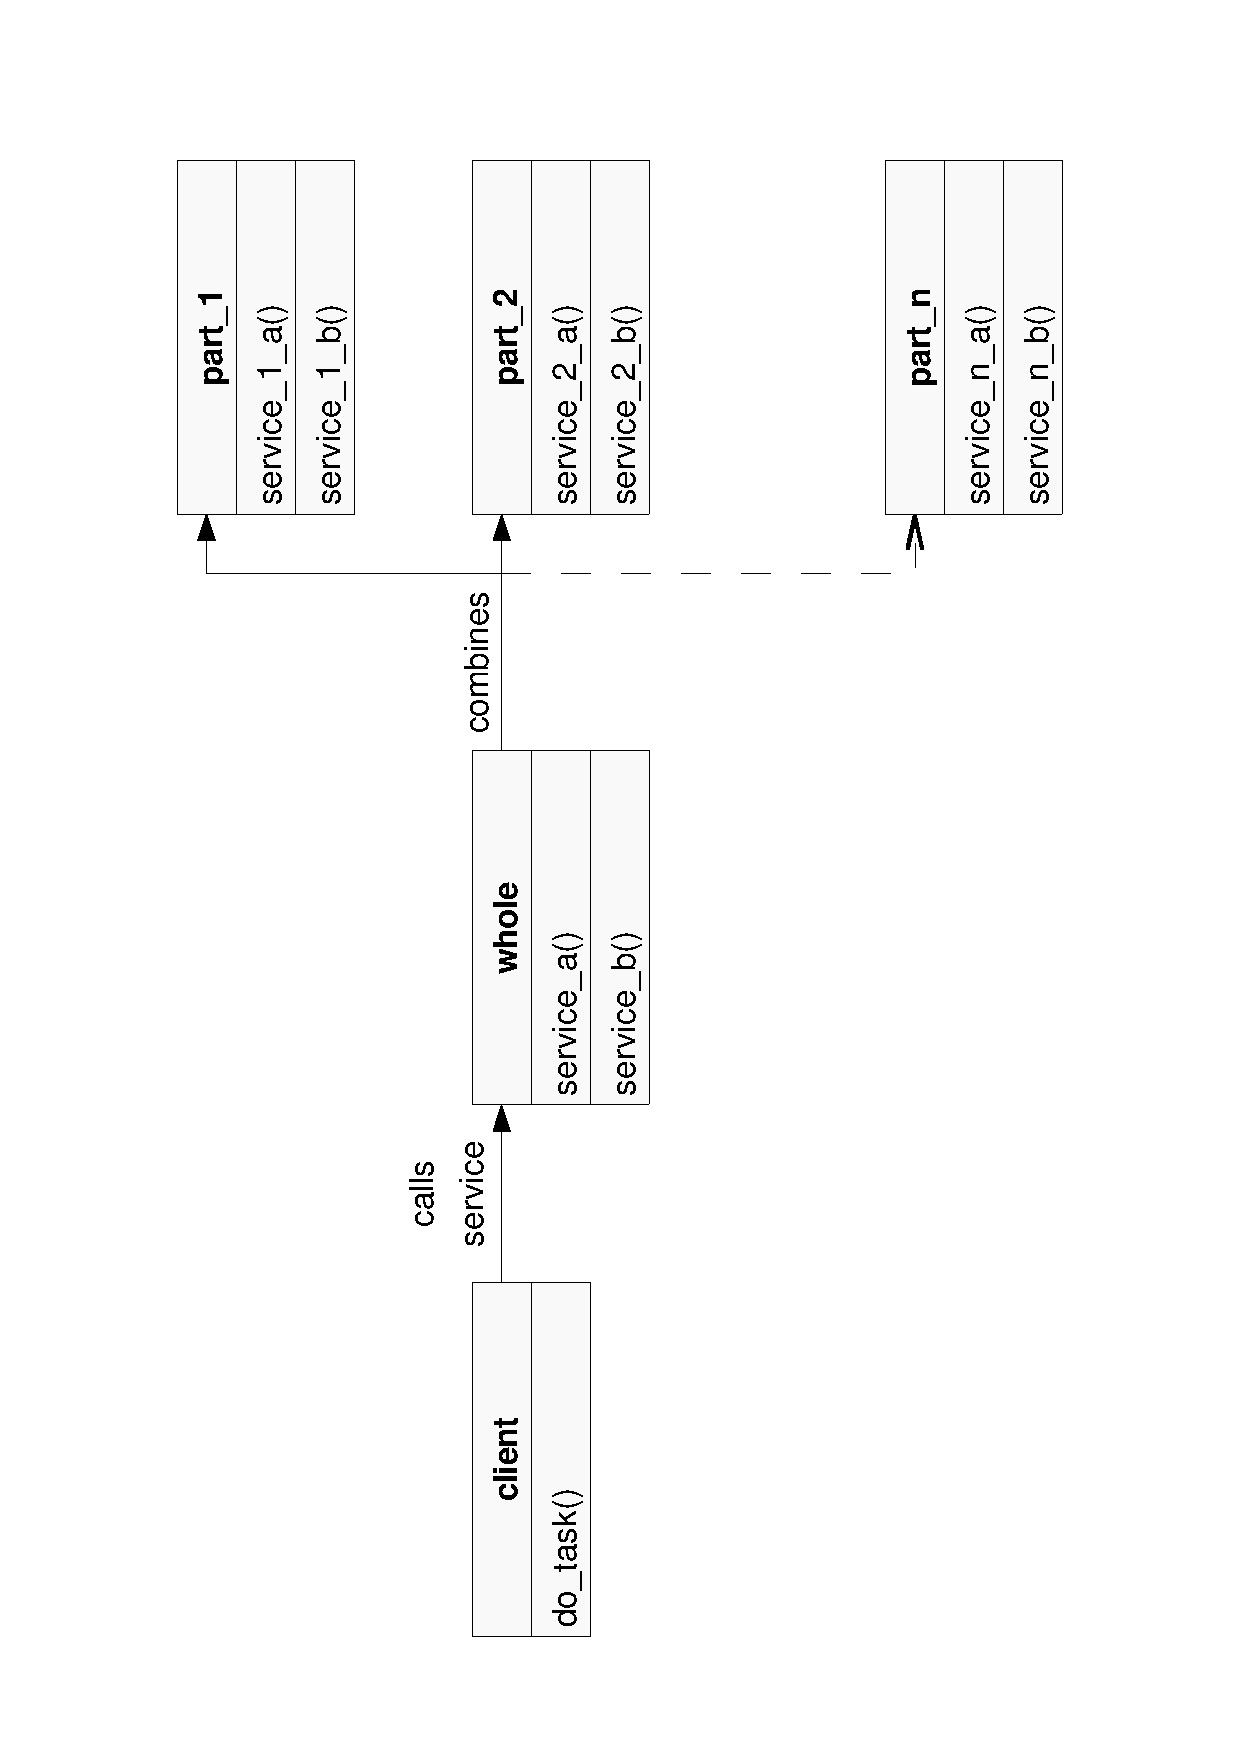
\includegraphics[scale=0.3,angle=-90]{graphic/wholepart.pdf}
        \caption{Whole-Part Pattern}
        \label{wholepart_figure}
    \end{center}
\end{figure}

The principal structure of the new language introduced in chapter
\ref{cybernetics_oriented_language_heading} is based on the \emph{Whole-Part}
pattern. One knowledge template (whole) may consist of zero, one or many other
templates (parts).
